%
%  untitled
%
%  Created by David Darmon on 2014-01-02.
%  Copyright (c) 2014 __MyCompanyName__. All rights reserved.
%
\documentclass[]{article}

% Use utf-8 encoding for foreign characters
\usepackage[utf8]{inputenc}

% Setup for fullpage use
\usepackage{fullpage}

% Uncomment some of the following if you use the features
%
% Running Headers and footers
%\usepackage{fancyhdr}

% Multipart figures
%\usepackage{subfigure}

% More symbols
%\usepackage{amsmath}
%\usepackage{amssymb}
%\usepackage{latexsym}

% Surround parts of graphics with box
\usepackage{boxedminipage}

% Package for including code in the document
\usepackage{listings}

% If you want to generate a toc for each chapter (use with book)
\usepackage{minitoc}

% This is now the recommended way for checking for PDFLaTeX:
\usepackage{ifpdf}

%\newif\ifpdf
%\ifx\pdfoutput\undefined
%\pdffalse % we are not running PDFLaTeX
%\else
%\pdfoutput=1 % we are running PDFLaTeX
%\pdftrue
%\fi

\ifpdf
\usepackage[pdftex]{graphicx}
\else
\usepackage{graphicx}
\fi
\title{}
\author{  }

\date{}

\begin{document}

\ifpdf
\DeclareGraphicsExtensions{.pdf, .jpg, .tif}
\else
\DeclareGraphicsExtensions{.eps, .jpg}
\fi

\maketitle

\begin{figure}[h!]
  \centering
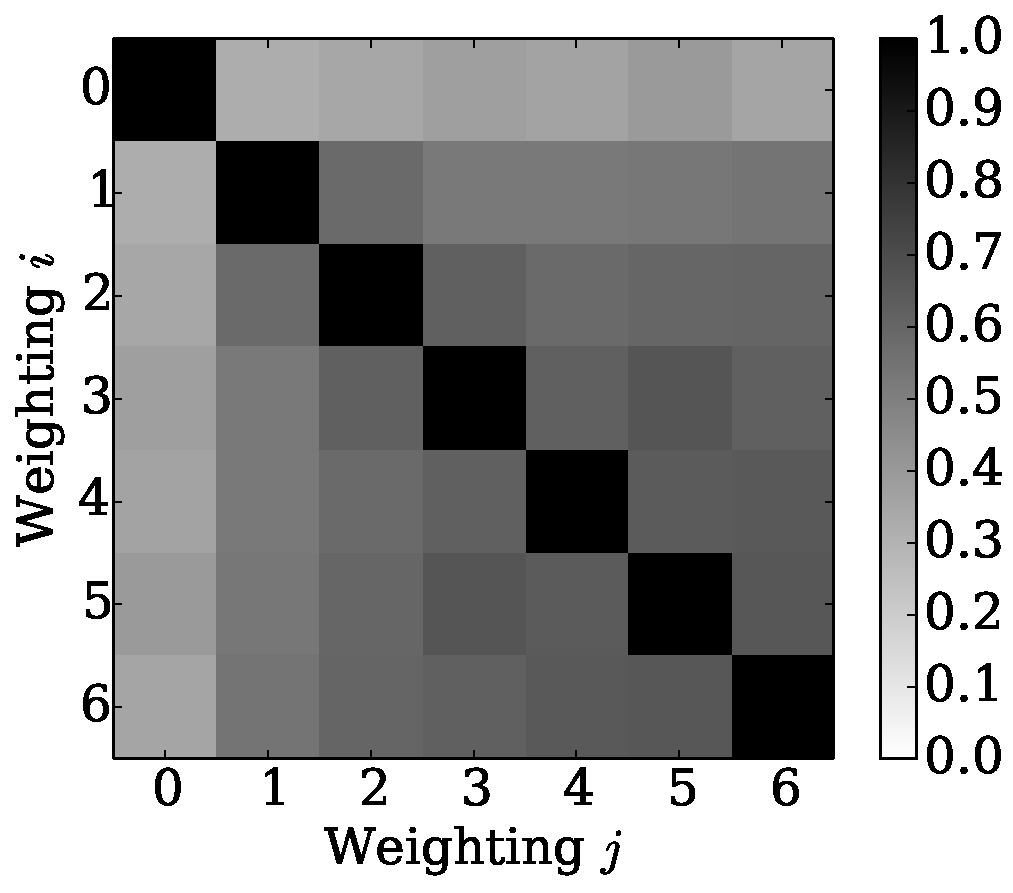
\includegraphics[width=0.50\textwidth]{Figures/nmi_singletons.pdf}
\caption{The normalized mutual information between the coverings for the communities determined using the structural $(i = j = 0)$ and transfer entropy (with lag $i, j \geq 1$) networks. A value of 1 for the normalized mutual information means that the coverings (i.e. communities) are identical.}
\label{Fig-}
\end{figure}

\begin{figure}[h!]
  \centering
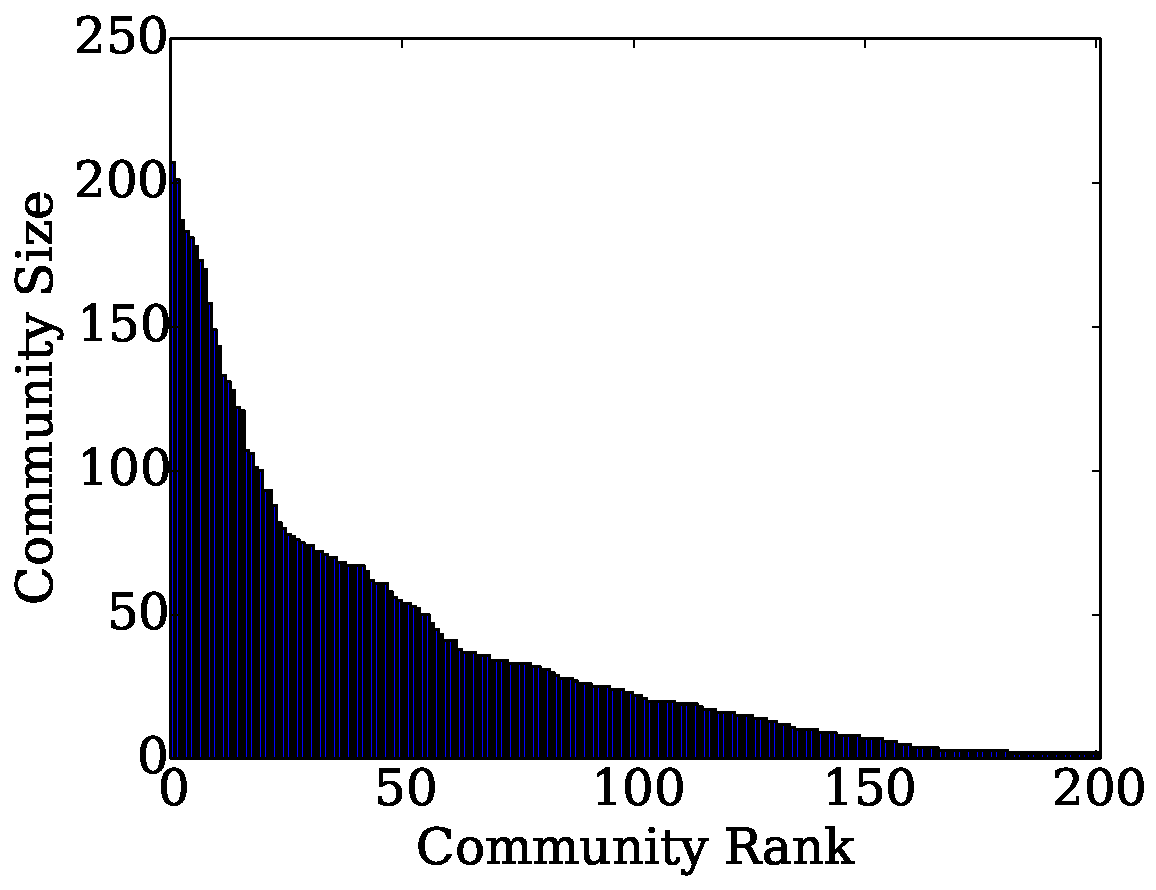
\includegraphics[width=0.50\textwidth]{Figures/comm-oslom0.pdf}
\caption{\textbf{Structural Network:} For each of the non-singleton communities, this shows the size of the community as a function of the rank of the community (in terms of size).}
\label{Fig-}
\end{figure}

\begin{figure}[h!]
  \centering
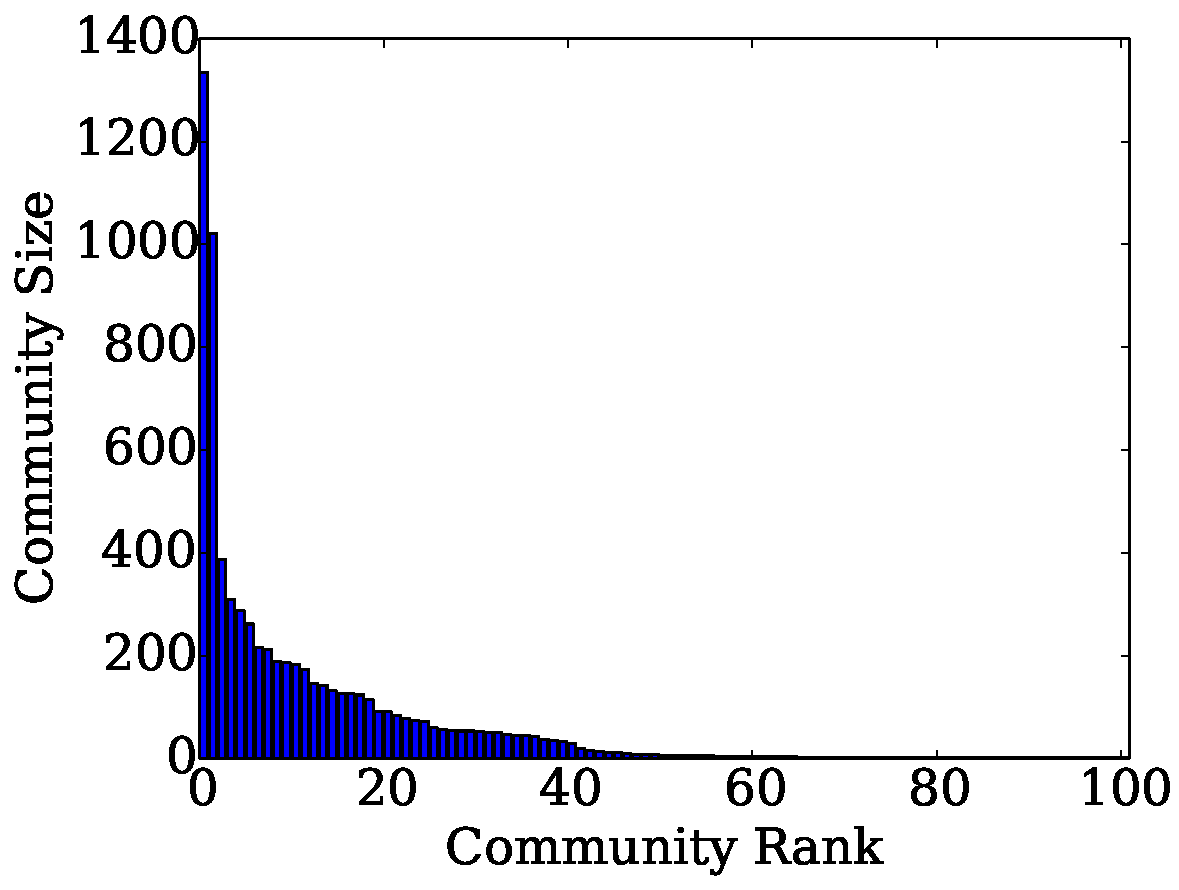
\includegraphics[width=0.50\textwidth]{Figures/comm-oslom1.pdf}
\caption{\textbf{Lag-1 Transfer Entropy Network:} For each of the non-singleton communities, this shows the size of the community as a function of the rank of the community (in terms of size).}
\label{Fig-}
\end{figure}

\begin{figure}[h!]
  \centering
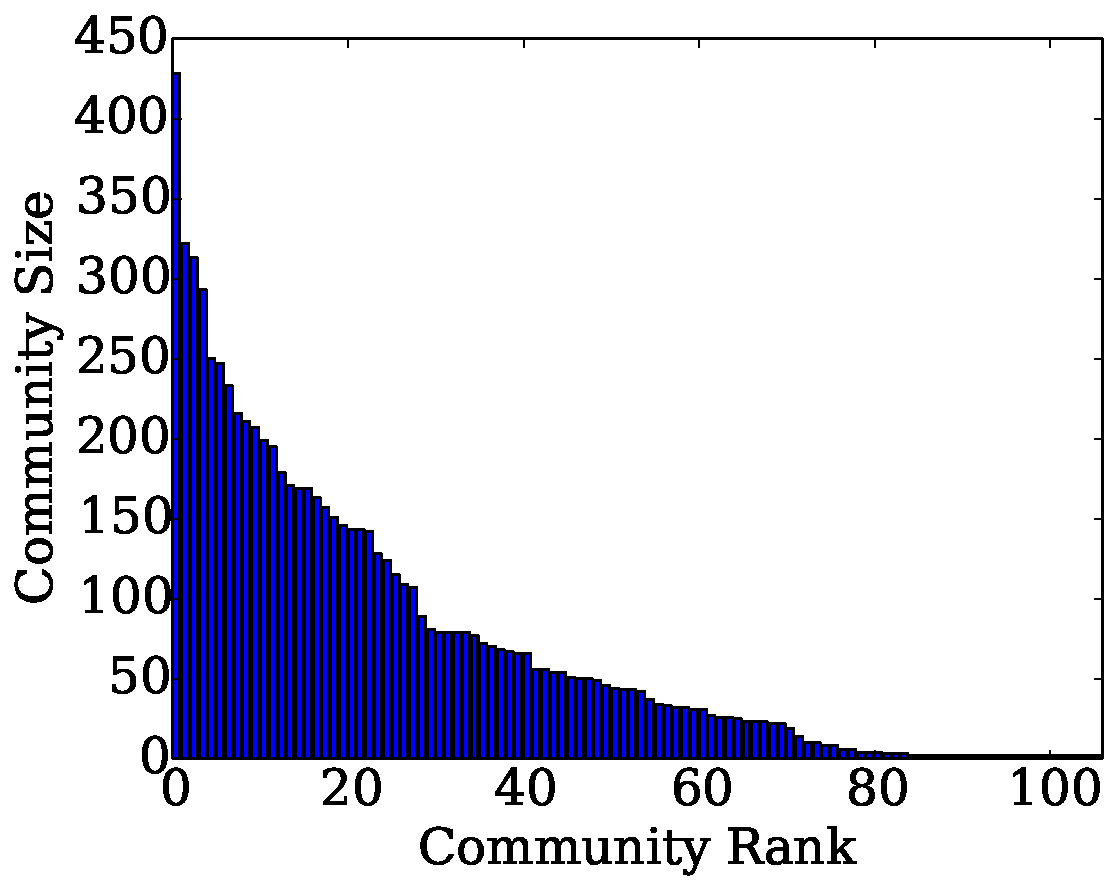
\includegraphics[width=0.50\textwidth]{Figures/comm-oslom3.pdf}
\caption{\textbf{Lag-3 Transfer Entropy Network:} For each of the non-singleton communities, this shows the size of the community as a function of the rank of the community (in terms of size).}
\label{Fig-}
\end{figure}

\begin{figure}[h!]
  \centering
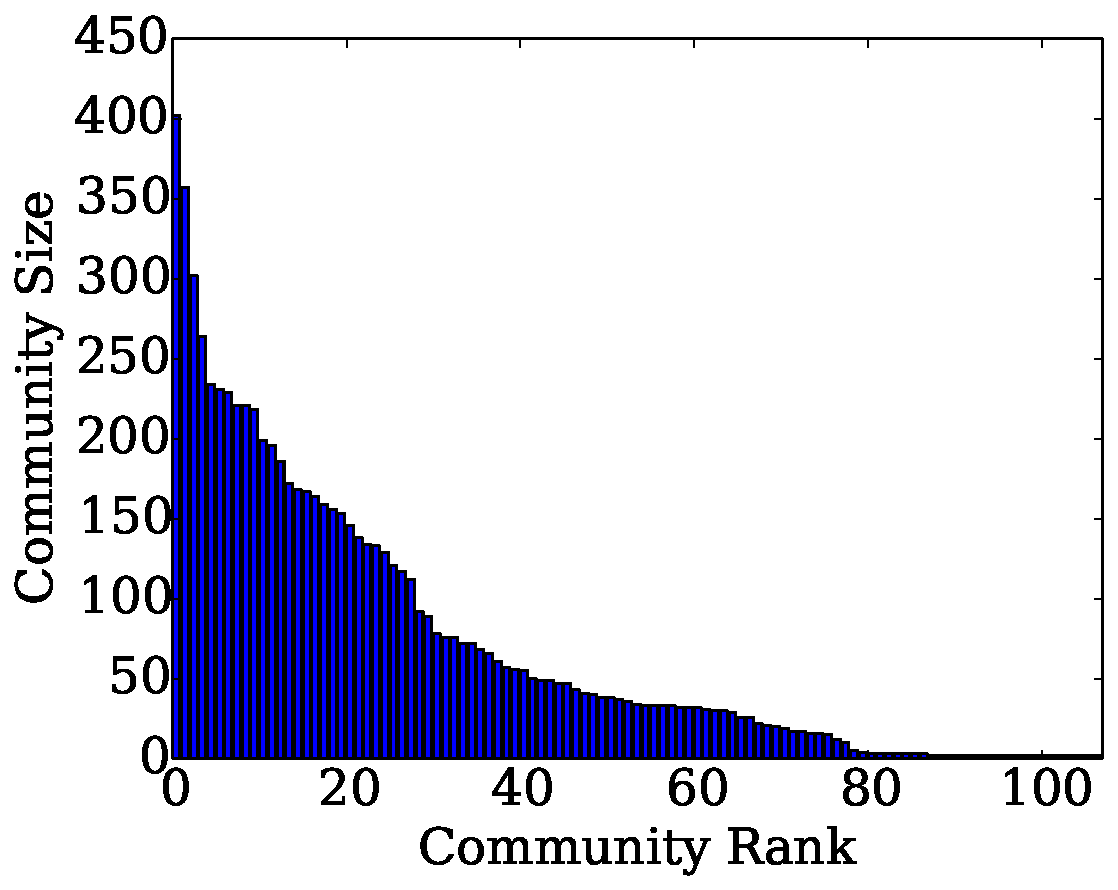
\includegraphics[width=0.50\textwidth]{Figures/comm-oslom5.pdf}
\caption{\textbf{Lag-5 Transfer Entropy Network:} For each of the non-singleton communities, this shows the size of the community as a function of the rank of the community (in terms of size).}
\label{Fig-}
\end{figure}

\begin{figure}[h!]
  \centering
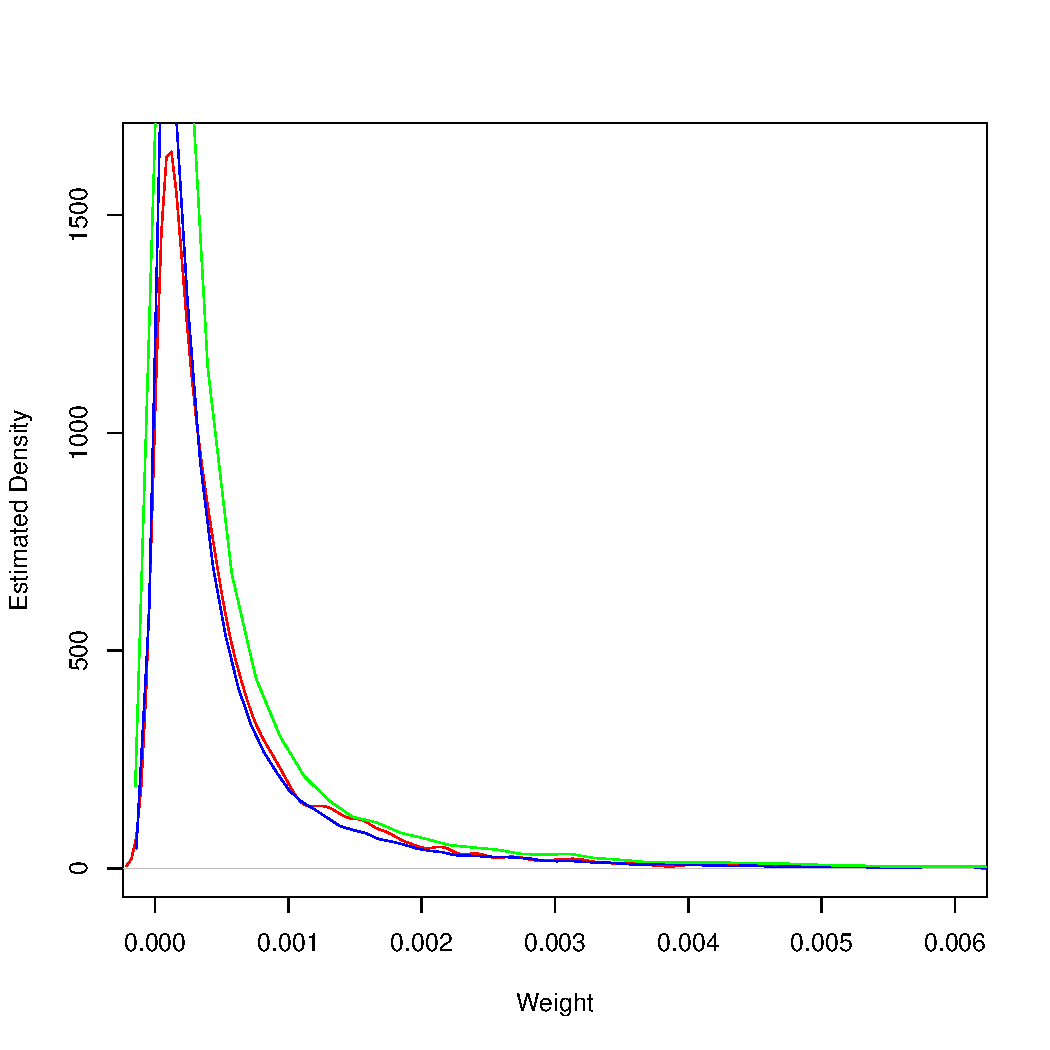
\includegraphics[width=0.50\textwidth]{Figures/comm78_labels-struc_weights-TE1-dens.pdf}
\caption{The empirical density for the weights on edges internal-to-internal (red), internal-to-external (green), and external-to-internal (blue) for community 78 using the communities determined by the structural network and the weights from the lag-1 transfer entropy community.}
\label{Fig-}
\end{figure}

\end{document}
